\documentclass{article}
\usepackage[spanish]{babel}
\usepackage{graphicx}
\usepackage{hyperref}

\title{AlephNull: Un Jugador Autónomo de Hex}
\author{Luis Ernesto Amat Cárdenas C-312}
\date{\today}

\begin{document}

\maketitle

\begin{abstract}
Este documento detalla el proceso de desarrollo de \textbf{AlephNull}, un agente autónomo para el juego Hex que combina técnicas de búsqueda heurística con optimizaciones algorítmicas. El jugador resultante supera consistentemente a oponentes básicos (aleatorios y greedy) y ofrece resistencia contra humanos.
\end{abstract}

\section{Objetivo}
Desarrollar un jugador de Hex que:
\begin{itemize}
\item Derrote consistentemente a oponentes automatizados
\item Minimice el número de movimientos para victoria (gane lo más rapido posible)
\item Mantenga competitividad contra jugadores humanos (sea entretenido)
\end{itemize}

\section{Metodología}
\subsection{Evolución del Algoritmo}
\begin{figure}[h]
\centering
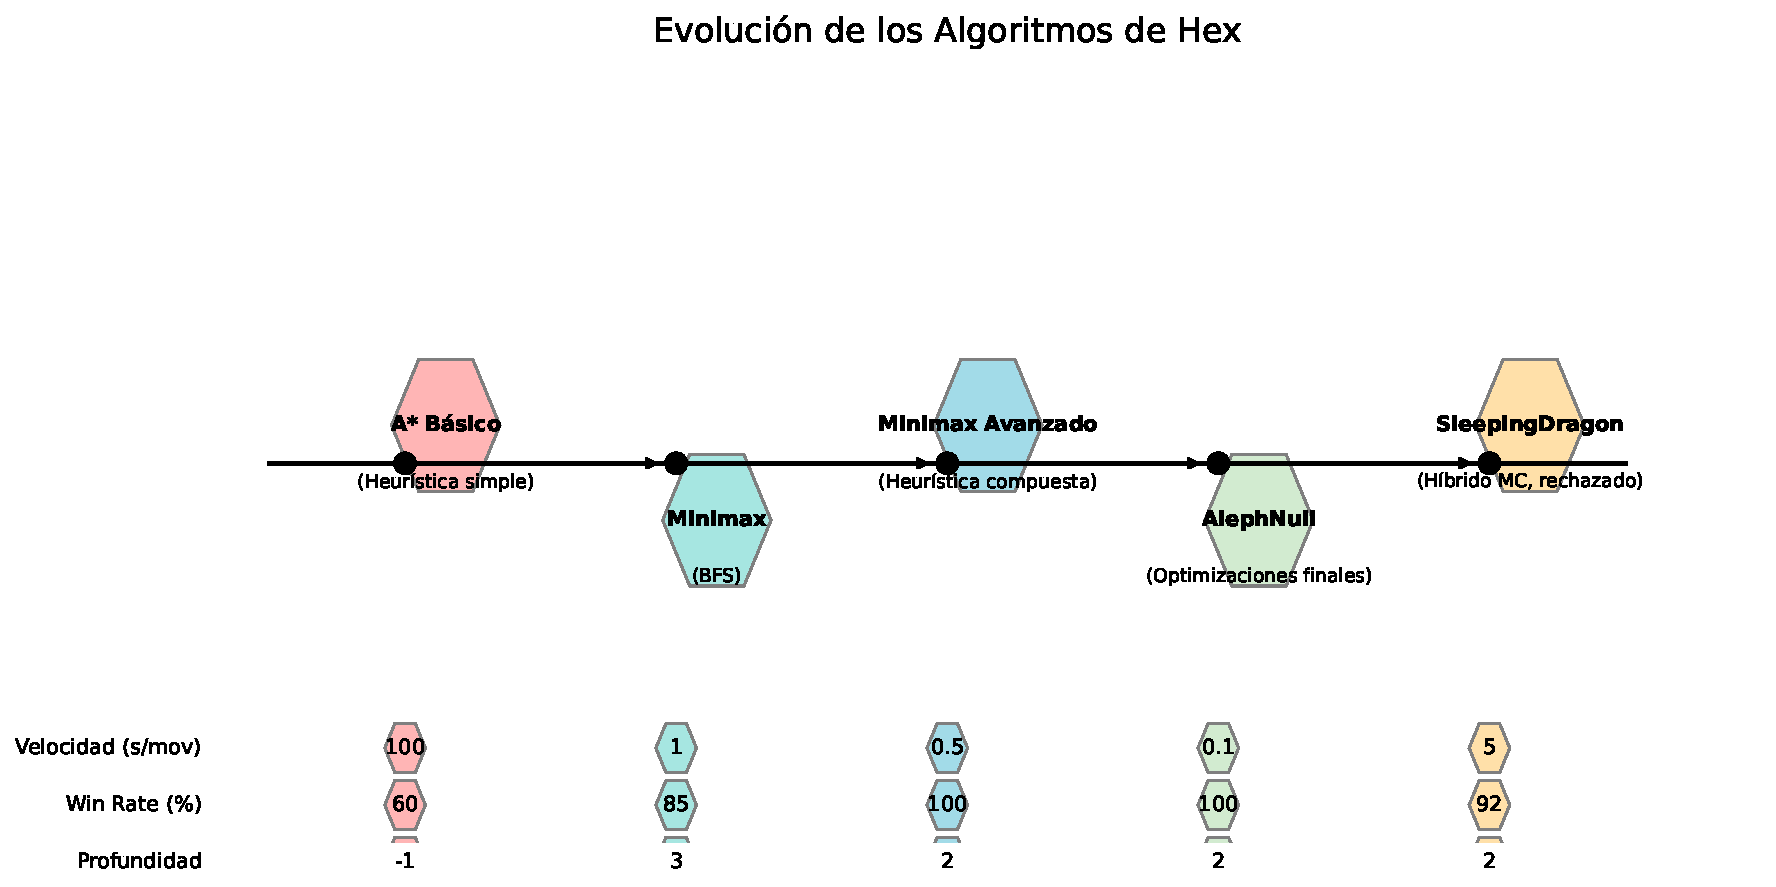
\includegraphics[width=0.8\textwidth]{evolucion_algoritmos.pdf}
\caption{Progresión de las versiones del jugador}
\end{figure}

\subsubsection*{Fase 1: A* Básico}
\begin{itemize}
\item Implementación inicial con heurística de camino más corto
\item Problemas: Complejidad temporal $O(b^d)$ inviable ($b \approx 121$ para tablero 11×11)
\item Logro: Base para la heurística de distancia optimizada
\end{itemize}

\subsubsection*{Fase 2: Minimax Temprano}
\begin{itemize}
\item Búsqueda de camino de costo mínimo a lo ancho
\item Heurística inicial:
\[ h(n) = d_{\text{victoria}} \]
\item Limitación: Enfoque naive sin estrategia ofensiva
\end{itemize}

\subsubsection*{Fase 3: Minimax Avanzado}
Heurística final con componentes:
\[ h(n) = \underbrace{2(s - d)}_{\text{Victoria}} + \underbrace{0.5c_1 + 0.2c_2}_{\text{Estructura}} + \underbrace{0.01o}_{\text{Defensa}} \]

Donde:
\begin{itemize}
\item $s$: Tamaño del tablero
\item $d$: Distancia del camino más corto (en particular, piezas faltantes en el camino de costo mínimo)
\item $c_n$: Piezas propias a distancia $n$ del camino
\item $o$: Piezas oponentes adyacentes al camino más corto (combinado con las otras heurísticas, causa que se bloquee al oponente en los "puentes")
\end{itemize}

En general, el jugador se dirige de un lado al otro del tablero lo más rapido posible mientras genera estructuras defensivas y se protege de ataques menores.
Las simulaciones indican que esta estrategia asegura la victoria en $s/2$ turnos \bfseries{de no ser interrumpida}.

\subsection{Abordajes Rechazados}
\begin{table}[h]
\centering
\begin{tabular}{|l|l|}
\hline
\textbf{Técnica} & \textbf{Razón de rechazo} \\
\hline
Heurística Manhattan & Incompatible con topología hexagonal (véase manhattan.pdf) \\
Híbrido Minimax-Monte-Carlo & Menos eficiente e inferior a Minimax puro\\
A* optimizado & Minimax superó en rendimiento \\
Reescritura de la heurística en C &  Rechazado en favor de pobar la efectividad de M-C\\
\hline
\end{tabular}
\end{table}

\section{Optimizaciones Clave}
\subsection{Representación del Grafo}
\begin{itemize}
\item \textbf{Nodos fantasma}: Conexiones virtuales a bordes opuestos para minimizar los cambios requeridos en el algoritmo
\item \textbf{Reinterpretación del grafo}: Eliminación de nodos oponentes en BFS y 'compresión' de los nodos propios (véase la estructura Árbol de Aristas Puentes donde se usa una técnica parecida).
\item Coste computacional reducido de $O(n^2)$ de Dijkstra a $O(V + E)$ de BFS
\end{itemize}

\subsection{Minimax con Alpha-Beta}
\begin{itemize}
\item Poda de gran parte de nodos en promedio
\end{itemize}

\section{Resultados}
\subsection{Métricas de Rendimiento}
\begin{table}[h]
\centering
\begin{tabular}{|l|c|c|}
\hline
\textbf{Oponente} & \textbf{Win Rate} & \textbf{Mov. Promedio} \\
\hline
Monke (Aleatorio) & 100\% & $s/2$ \\
Usagi (Greedy) & 100\% & $s/2$ \\
M-C (players probados) & 100\% & $s/2$ \\
\hline
\end{tabular}
\end{table}

\subsection{Conclusiones}
\begin{itemize}
\item Una heurística bien balanceada supera a búsquedas no informadas al inicio
\item La estructura de puentes temprana es crucial
\item Es mejor algoritmo es el que gana más (y mejor aún que si gana rápido)
\item La paralelización beneficia más a Monte Carlo que a Minimax
\item El enfoque híbrido no siempre proporciona ventajas
\end{itemize}

\begin{thebibliography}{9}
\bibitem{minimax} Knuth, D. \textit{Analysis of Alpha-Beta Pruning}. 1975.
\end{thebibliography}

\end{document}
